\documentclass[a4paper,12pt]{article}
\usepackage{tikz}
\usetikzlibrary{circuits.logic.US}
\usepackage{graphicx} % Required for inserting images
\usepackage{amsmath,amssymb,amsfonts}
\usepackage{subcaption}
% Use Times New Roman font
\usepackage{times}
\usepackage[a4paper, top=1in, bottom=0.8in, left=1.1in, right=0.8in]{geometry}
\usepackage{float}
\usepackage{listings}
\usepackage{xcolor} % For customizing code colors
\setlength{\parindent}{0pt}
\usepackage{titlesec} % Add this to your preamble
\titleformat{\section}
{\normalfont\large\bfseries}{\thesection}{1em}{}
% Set spacing for sections
\titlespacing*{\section}
{0pt}  % Left spacing
{1ex} % Space before (adjust this value)
{1ex}  % Space after (adjust this value)
\begin{document}
	\section{Experiment No. 9}
	
	
	\section{Experiment Title }
	Design and Analyze of 2$\times$1 and 4$\times$1 MUX on MICROWIND 3.0.
	\section{Objective}
	The main objectives of this report are:
	\begin{itemize}
		 \item To understand the working principle of a transmission gate.
		\item To design and simulate 2$\times$1 , 4$\times$1 MUX on MICROWIND 3.0.
	
	\end{itemize}
	\section{Theory}
	
	The circuit shown is a \textbf{transmission gate}, which consists of a pMOS and an nMOS transistor connected in parallel. It is controlled by complementary signals \(S\) and \(\overline{S}\).
	
	\subsection*{Working Principle}
	\begin{enumerate}
		\item \textbf{Inputs and Outputs:}
		\begin{enumerate}
			\item \textbf{Input (\(A\))}: Signal to be transmitted.
			\item \textbf{Output (\(Y\))}: Signal after passing through the transmission gate.
			\item \textbf{Control Signals (\(S\) and \(\overline{S}\))}:
		
			\(S\) is the control signal	, \(\overline{S}\) is the complement of \(S\).
	
		\end{enumerate}
			\begin{table}[H]
			\centering
			\begin{tabular}{|c|c|c|}
				\hline
				\begin{tabular}[c]{@{}c@{}} \\ $\bar{S}$\\  \end{tabular} & \begin{tabular}[c]{@{}c@{}} \\ $S$\\  \end{tabular} & \begin{tabular}[c]{@{}c@{}} \\ Output (Y)\\  \end{tabular} \\ \hline
				1                                                         & 0                                                   & A                                                              \\ \hline
				0                                                         & 1                                                   & N$\backslash$A                                                             \\ \hline
			\end{tabular}
		\end{table}
		\item \textbf{Operation:}
		\begin{enumerate}
			\item When \(S = 1\) and \(\overline{S} = 0\):
			\begin{enumerate}
				\item Both nMOS and pMOS are \textbf{ON}.
				\item The input \(A\) is passed to the output \(Y\) with minimal resistance.
			\end{enumerate}
			
			\item When \(S = 0\) and \(\overline{S} = 1\):
			\begin{enumerate}
				\item Both nMOS and pMOS are \textbf{OFF}.
				\item The input \(A\) is disconnected from the output \(Y\).
			\end{enumerate}
		\end{enumerate}
	\end{enumerate}

	
	\begin{figure}[H]
		\centering
		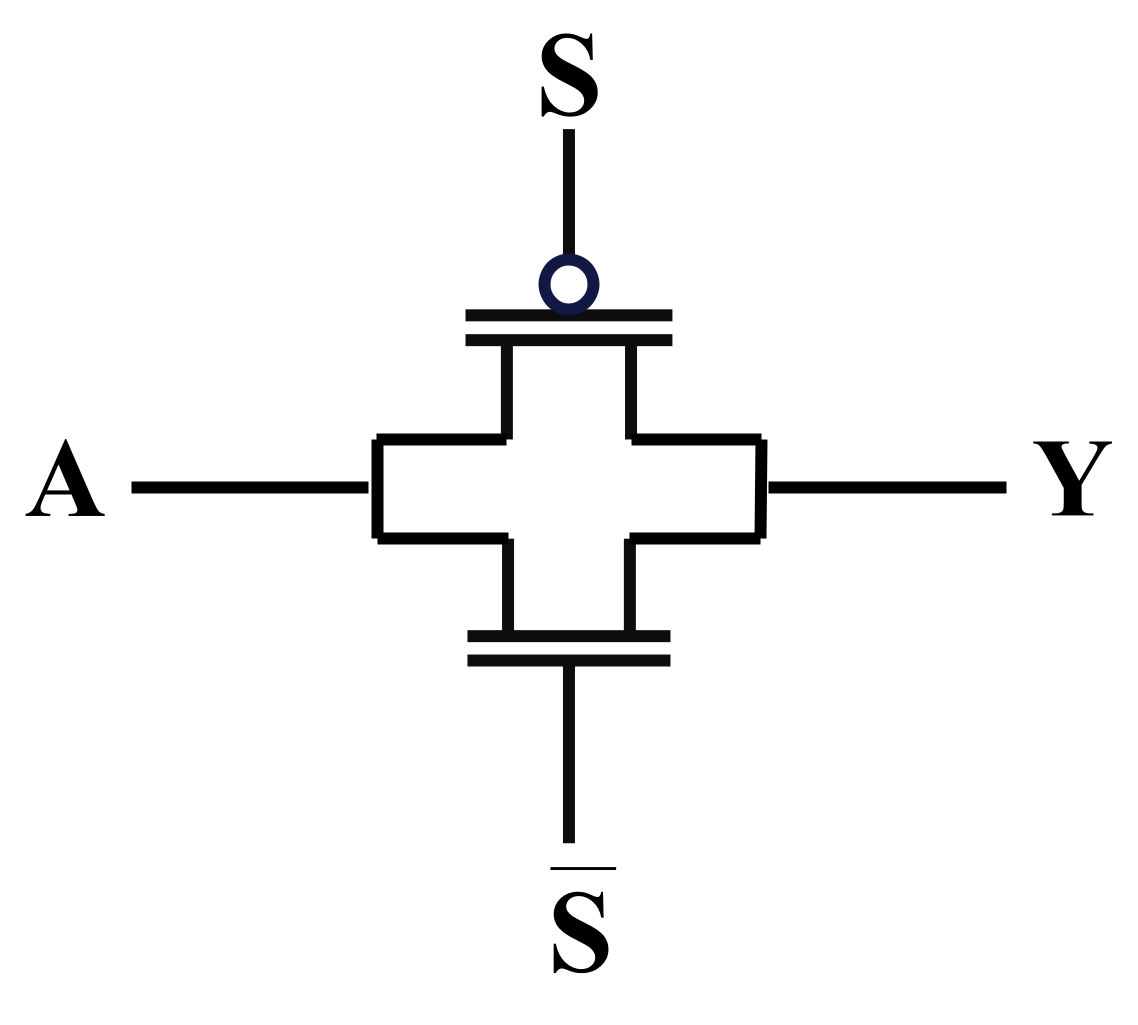
\includegraphics[width=0.32\linewidth]{Images/tgate}
		\caption{ Transmission Gate}
		\label{fig:1}
	\end{figure}
\newpage
	\subsection{2x1 Multiplexer}

A multiplexer is a combinational circuit that selects one of many input signals and forwards the selected input to a single output line. A 2x1 multiplexer has two input lines (A and B), one select line (S), and one output line (Y).

\subsubsection{Working Principle}
The output of the 2x1 multiplexer is given by the Boolean equation:
\[
Y = \overline{S} \cdot A + S \cdot B
\]


	
	A 2x1 multiplexer selects one of two input signals (\(A\) or \(B\)) based on a control signal (\(S\)) and outputs the selected input to \(Y\). The working process is as follows:
	
	\begin{table}[H]
		\centering
		\begin{tabular}{|c|c|c|}
			\hline
			\begin{tabular}[c]{@{}c@{}} \\ $\bar{S}$\\  \end{tabular} & \begin{tabular}[c]{@{}c@{}} \\ $S$\\  \end{tabular} & \begin{tabular}[c]{@{}c@{}} \\ Selected Input\\  \end{tabular} \\ \hline
			1                                                         & 0                                                   & A                                                              \\ \hline
			0                                                         & 1                                                   & B                                                              \\ \hline
		\end{tabular}
	\end{table}
		Below is the simplified transistor-level implementation of a 2x1 multiplexer:
	\begin{figure}[H]
		\centering
		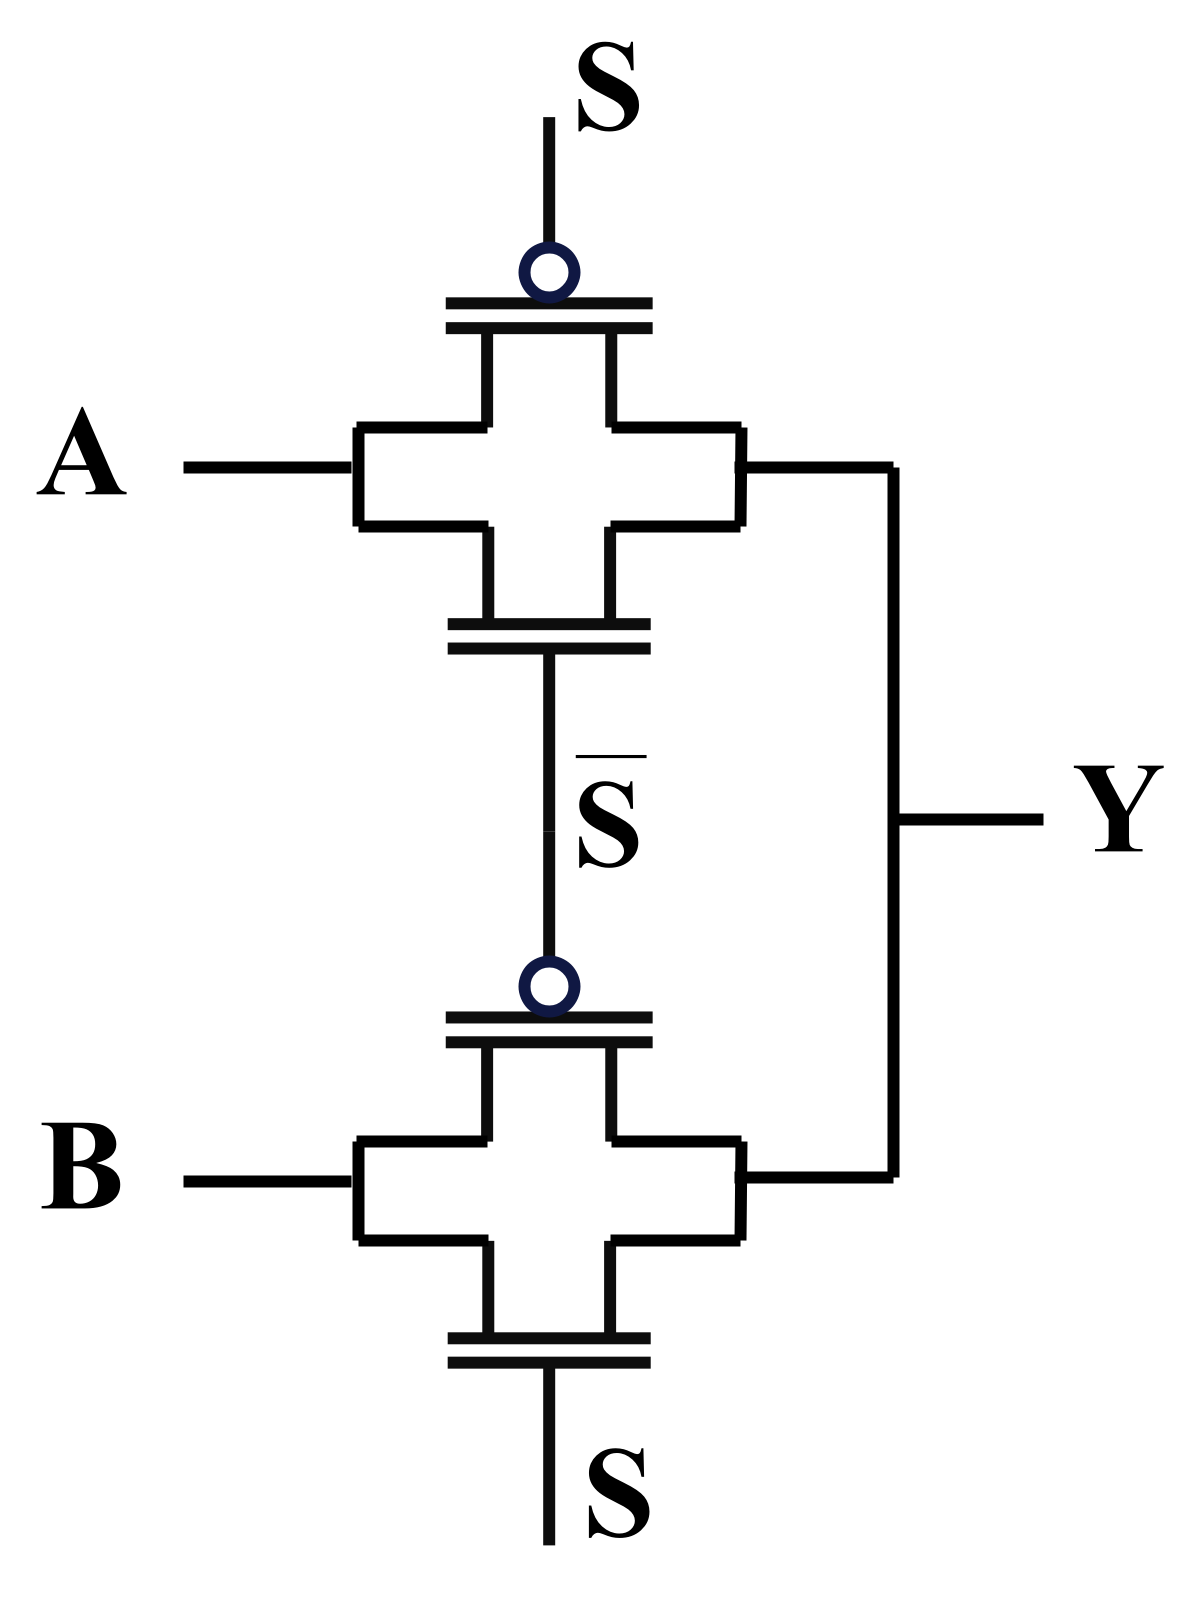
\includegraphics[width=0.30\linewidth]{Images/2x1}
		\caption{2$\times$1 Multiplexer Design using Transmission Gate}
		\label{fig:1}
	\end{figure}
	\textbf{When S = 0:}
	\begin{itemize}
		\item The input \(A\) is selected, and its value is passed to the output \(Y\).
		\item This happens because the top pMOS transistor (controlled by \(S\)) turns \textbf{ON}, allowing \(A\) to pass to the output.
	\end{itemize}
	
\textbf{	When S = 1:}
	\begin{itemize}
		\item The input \(B\) is selected, and its value is passed to the output \(Y\).
		\item In this case, the bottom pMOS transistor (controlled by \(S\)) turns \textbf{ON}, enabling \(B\) to pass to the output.
	\end{itemize}
	
	This multiplexer uses complementary logic to ensure that only one path is active at a time.
	
	
	
	\newpage
		\subsection{4x1 Multiplexer}

	
	A 4x1 multiplexer is a combinational circuit that selects one of four input signals (\(A\), \(B\), \(C\), or \(D\)) based on two control signals (\(S_1\) and \(S_0\)) and outputs the selected input to \(Y\). This implementation uses transmission gates for efficient signal selection.\\
	The selection process depends on the control signals as shown in the truth table below:
	
	\[
	\begin{array}{|c|c|c|}
		\hline
		S_0 & S_1 & \text{Selected Input} \\ \hline
		0   & 0   & A \\ \hline
		0   & 1   & C \\ \hline
		1   & 0   & B \\ \hline
		1   & 1   & D \\ \hline
	\end{array}
	\]
	\begin{figure}[H]
		\centering
		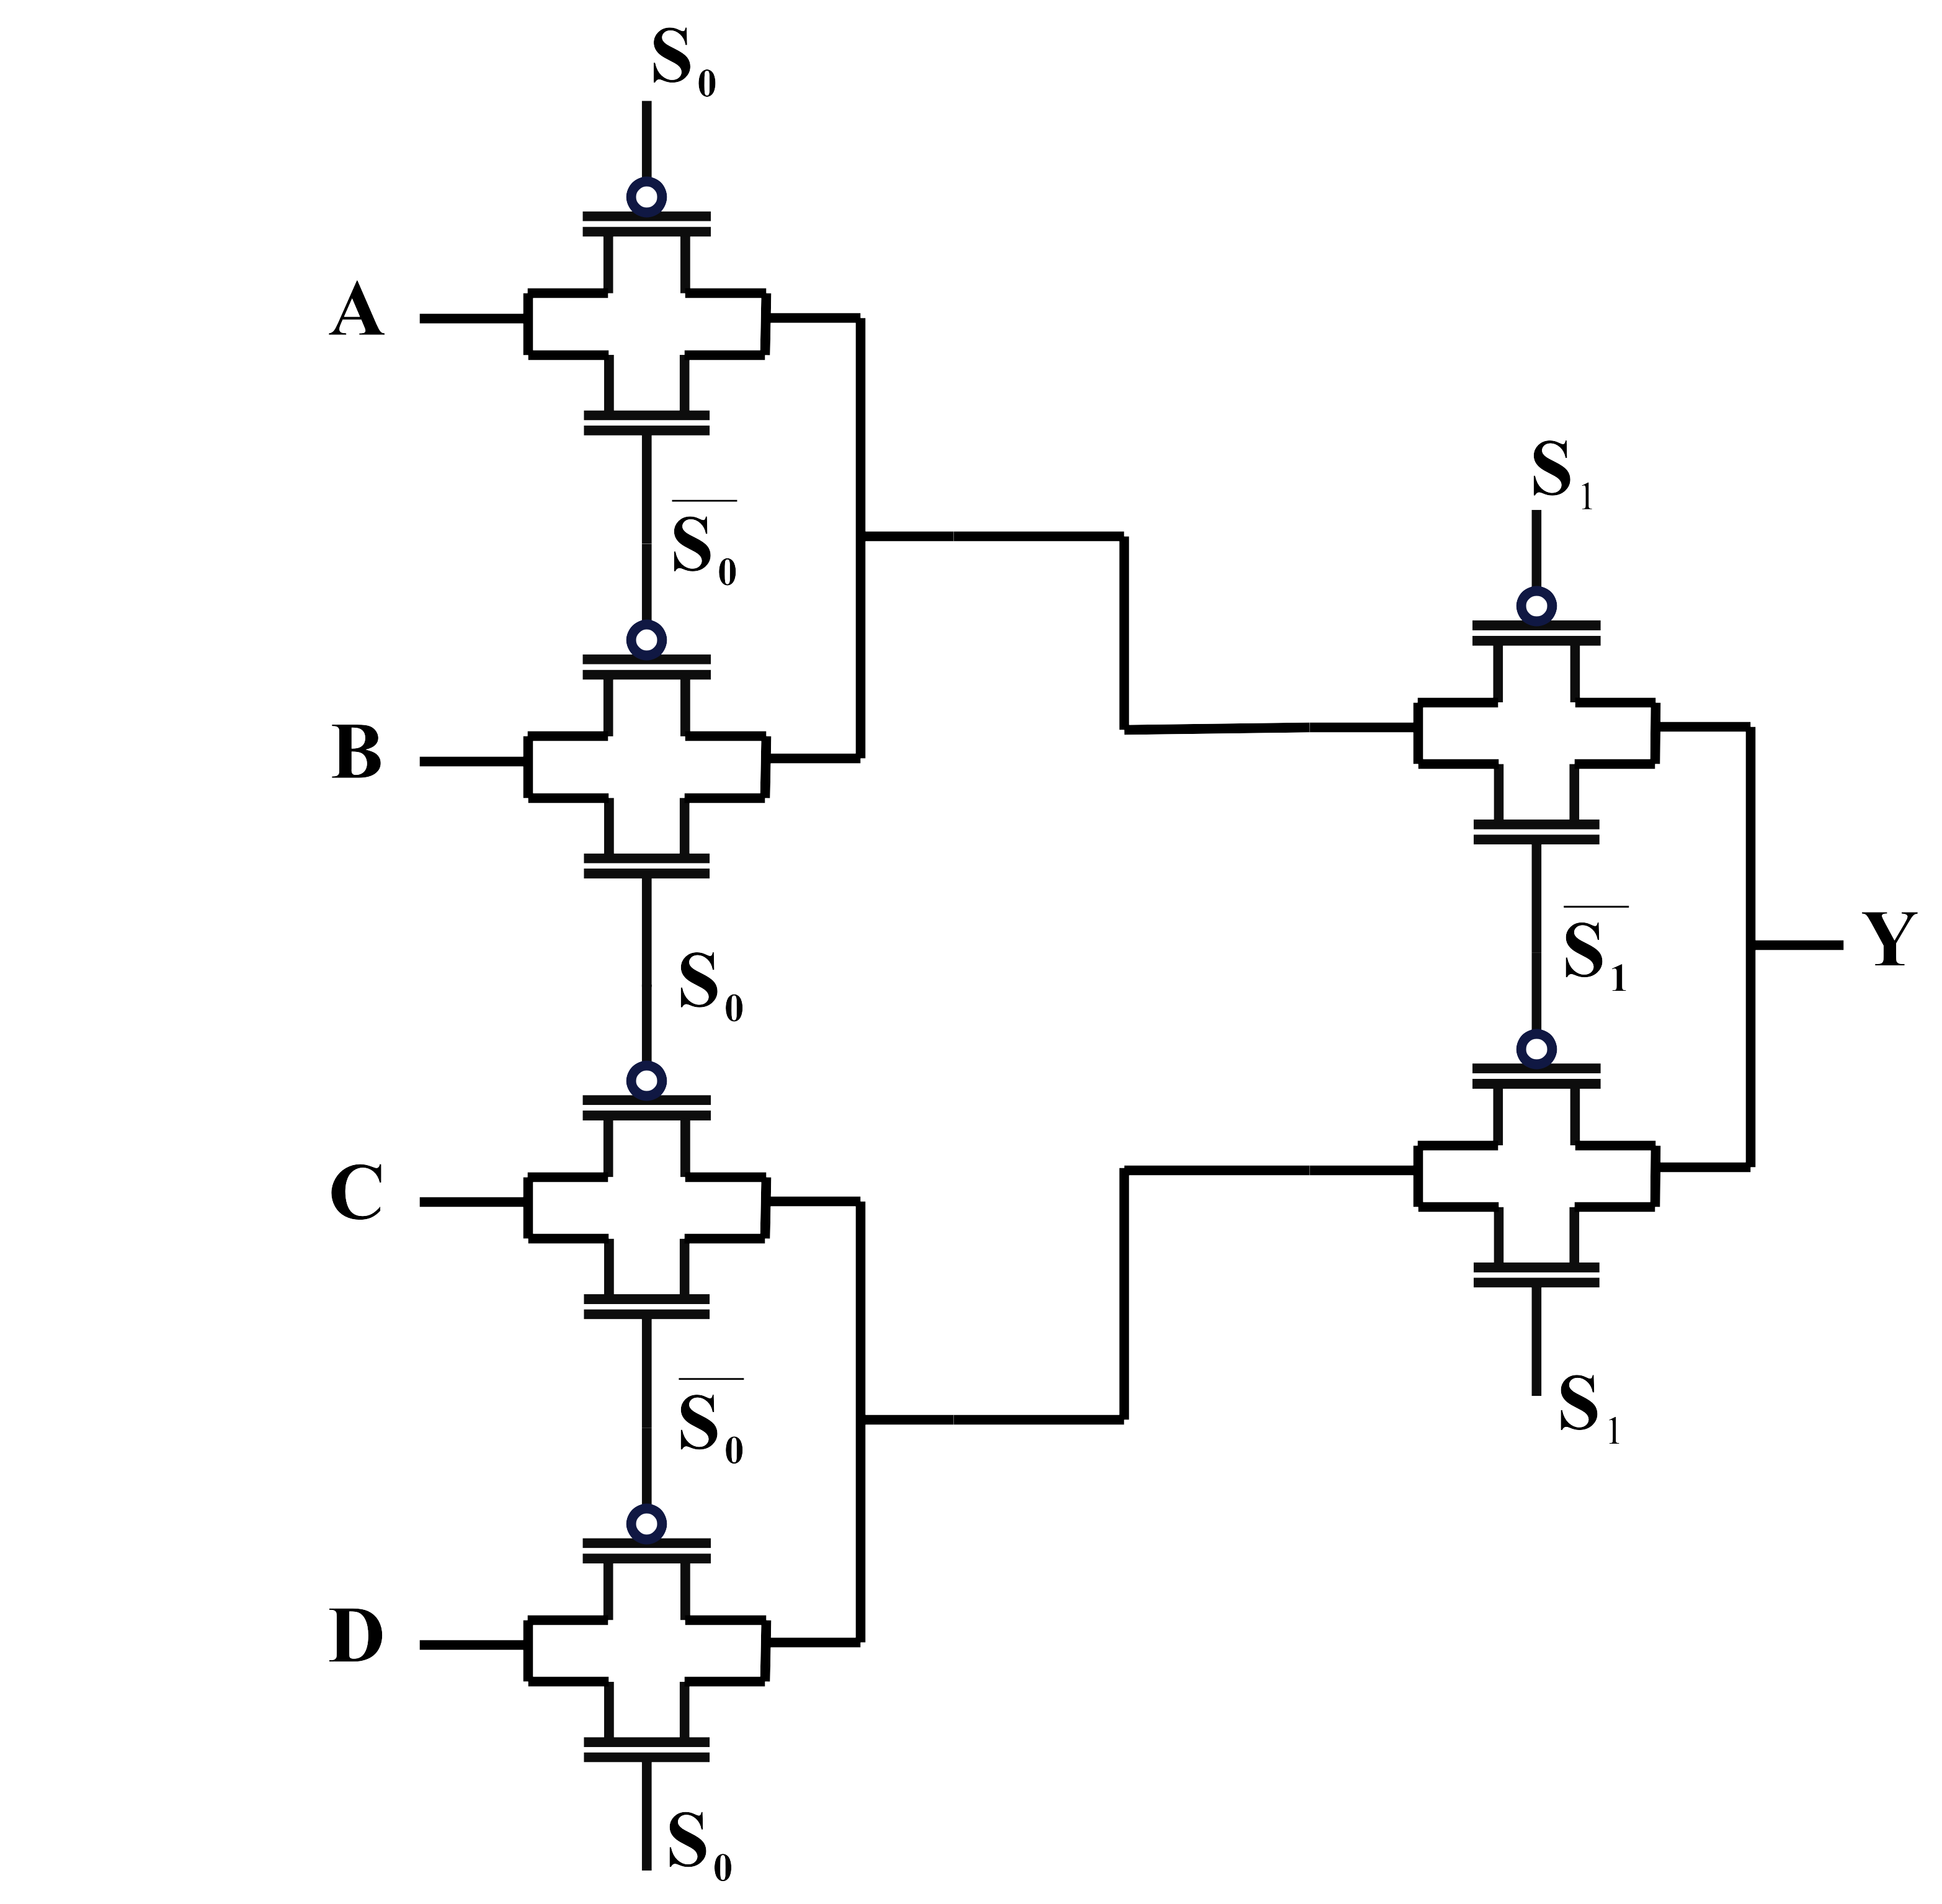
\includegraphics[width=0.7\linewidth]{Images/041}
			\caption{4$\times$1 Multiplexer Design using Transmission Gate}
		\label{fig:1}
	\end{figure}
\textbf{Working of 4x1 Multiplexer using Transmission Gates}
	\begin{itemize}
		\item \textbf{When \(S_1 = 0\) and \(S_0 = 0\):} The transmission gate connected to input \(A\) is activated, allowing \(A\) to pass to the output \(Y\).
		\item \textbf{When \(S_0 = 0\) and \(S_1 = 1\):} The transmission gate connected to input \(C\) is activated, allowing \(C\) to pass to the output \(Y\).
		\item \textbf{When \(S_0 = 1\) and \(S_1 = 0\):} The transmission gate connected to input \(B\) is activated, allowing \(B\) to pass to the output \(Y\).
		\item \textbf{When \(S_0 = 1\) and \(S_1 = 1\):} The transmission gate connected to input \(D\) is activated, allowing \(D\) to pass to the output \(Y\).
	\end{itemize}
	


	
	
	
	\newpage
	\section{Schematic Layout }
	\subsection{2$\times$1 Multiplexer}
\begin{figure}[H]
	\centering
	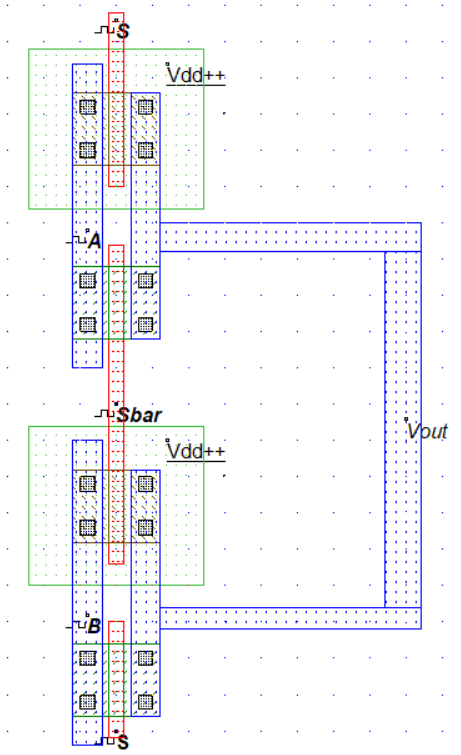
\includegraphics[width=0.7\linewidth]{Images/1}
	\caption{2$\times$1 Multiplexer Design }
	\label{fig:1}
\end{figure}
\subsection{4$\times$1 Multiplexer}
	\begin{figure}[H]
		\centering
		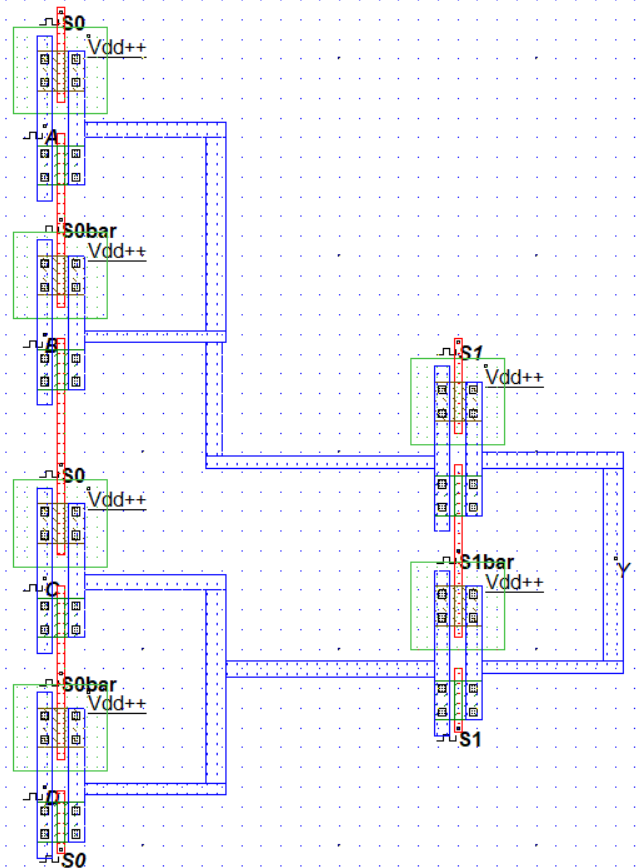
\includegraphics[width=1\linewidth]{Images/3}
		\caption{4$\times$1 Multiplexer Design }
		\label{fig:1}
	\end{figure}
	\subsection{4$\times$1 Multiplexer using nMOS Pass-Transistors}
	\begin{figure}[H]
		\centering
		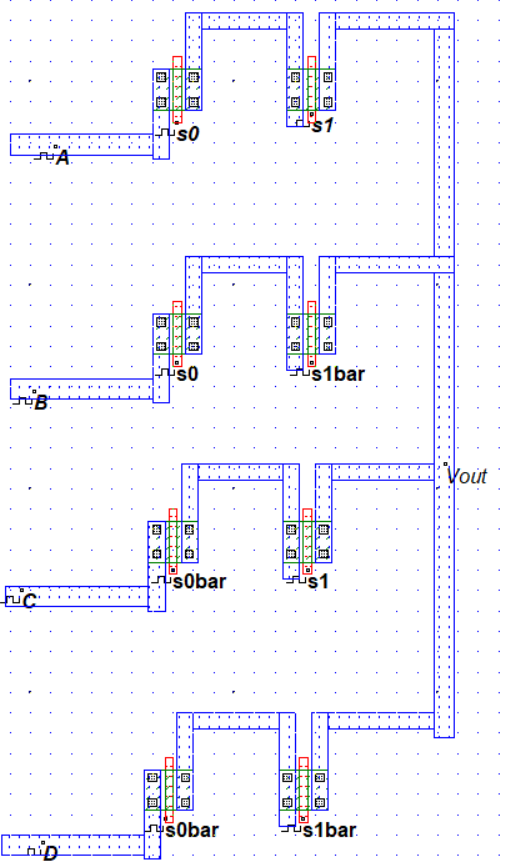
\includegraphics[width=0.81\linewidth]{Images/6}
		\caption{4$\times$1 Multiplexer Design using nMOS Pass-Transistors}
		\label{fig:1}
	\end{figure}
	\newpage
	
	\section{Specification}
		\begin{table}[H]
		\centering
		\caption{MOSFET Dimensions for nMOS and pMOS Transistors}
		\label{tab:MOSFET_dimensions}
		\begin{tabular}{|c|c|c|c|c|}
			\hline
			\textbf{MOS} & \textbf{\begin{tabular}[c]{@{}c@{}}Width\\ ($\mu m$)\end{tabular}} & \textbf{\begin{tabular}[c]{@{}c@{}}Length\\ ($\mu m$)\end{tabular}} & \textbf{\begin{tabular}[c]{@{}c@{}}Width\\ ($\lambda$)\end{tabular}} & \textbf{\begin{tabular}[c]{@{}c@{}}Length\\ ($\lambda$)\end{tabular}} \\ \hline
			nMOS & 0.600 & 0.120 & 10 & 2 \\ \hline
			pMOS & 0.600 & 0.120 & 10 & 2 \\ \hline
		\end{tabular}
		
	\end{table}
	\subsection{ 2$\times$1 Multiplexer}
		\begin{table}[H]
		\centering
		\caption{Parameters of Input Clock Signals for A,B S0 \& S0bar}
		% Sub-table (a)
		\begin{subtable}[t]{0.48\textwidth} % Adjusted width for each sub-table
			\centering
			\begin{tabular}{|c|c|c|}
				\hline
				\textbf{Parameter}          & \textbf{Value} & \textbf{Unit} \\ \hline
				High Level $(V)$            & 5.00           & $V$           \\ \hline
				Low Level $(V)$             & 0.00           & $V$           \\ \hline
				Time Low $(tl)$             & 0.225          & $ns$          \\ \hline
				Rise Time $(tr)$            & 0.002          & $ns$          \\ \hline
				Time High $(th)$            & 0.225          & $ns$          \\ \hline
				Fall Time $(tf)$            & 0.002          & $ns$          \\ \hline
			\end{tabular}
			\caption{Input clock signal of A} % Sub-table (a) caption
		\end{subtable}
		\hfil
		% Sub-table (b)
		\begin{subtable}[t]{0.48\textwidth} % Adjusted width for each sub-table
			\centering
			\begin{tabular}{|c|c|c|}
				\hline
				\textbf{Parameter}          & \textbf{Value} & \textbf{Unit} \\ \hline
				High Level $(V)$            & 5.00           & $V$           \\ \hline
				Low Level $(V)$             & 0.00           & $V$           \\ \hline
				Time Low $(tl)$             & 0.452         & $ns$          \\ \hline
				Rise Time $(tr)$            & 0.002          & $ns$          \\ \hline
				Time High $(th)$            & 0.452          & $ns$          \\ \hline
				Fall Time $(tf)$            & 0.002          & $ns$          \\ \hline
			\end{tabular}
			\caption{Input clock signal of B} % Sub-table (b) caption
		\end{subtable}
		
		\begin{subtable}[t]{0.48\textwidth} % Adjusted width for each sub-table
			\centering
			\begin{tabular}{|c|c|c|}
				\hline
				\textbf{Parameter}          & \textbf{Value} & \textbf{Unit} \\ \hline
				High Level $(V)$            & 5.00           & $V$           \\ \hline
				Low Level $(V)$             & 0.00           & $V$           \\ \hline
				Time Low $(tl)$             & 0.450         & $ns$          \\ \hline
				Rise Time $(tr)$            & 0.002          & $ns$          \\ \hline
				Time High $(th)$            & 0.450          & $ns$          \\ \hline
				Fall Time $(tf)$            & 0.002          & $ns$          \\ \hline
			\end{tabular}
			
			\caption{Input clock signal of S0} % Sub-table (a) caption
		\end{subtable}
		\hfil
		\begin{subtable}[t]{0.48\textwidth} % Adjusted width for each sub-table
			\centering
			\begin{tabular}{|c|c|c|}
				\hline
				\textbf{Parameter}          & \textbf{Value} & \textbf{Unit} \\ \hline
				High Level $(V)$            & 0.00           & $V$           \\ \hline
				Low Level $(V)$             & 5.00           & $V$           \\ \hline
				Time Low $(tl)$             & 0.450          & $ns$          \\ \hline
				Rise Time $(tr)$            & 0.002          & $ns$          \\ \hline
				Time High $(th)$            & 0.450         & $ns$          \\ \hline
				Fall Time $(tf)$            & 0.002          & $ns$          \\ \hline
			\end{tabular}
			
			\caption{Input clock signal of S0bar} % Sub-table (a) caption
		\end{subtable}
	\end{table}
	
	\begin{table}[H]
		\centering
		\caption{Parameters for Vdd+ and Vss- }
		\begin{tabular}{|c|c|c|}
			\hline
			\textbf{Parameter} & \textbf{Value} & \textbf{Unit} \\ \hline
			Vdd+               & 5.00           & $V $            \\ \hline
			Vss-               & 0.00           & $V$             \\ \hline
		\end{tabular}
		
	\end{table}
	\subsection{4$\times$1 Multiplexer}
	
	
	\begin{table}[H]
		\centering
		\caption{Parameters of Input Clock Signals for A,B,C,D S0, S0bar, S1 \& S1bar}
		% Sub-table (a)
		\begin{subtable}[t]{0.48\textwidth} % Adjusted width for each sub-table
			\centering
			\begin{tabular}{|c|c|c|}
				\hline
				\textbf{Parameter}          & \textbf{Value} & \textbf{Unit} \\ \hline
				High Level $(V)$            & 5.00           & $V$           \\ \hline
				Low Level $(V)$             & 0.00           & $V$           \\ \hline
				Time Low $(tl)$             & 0.225          & $ns$          \\ \hline
				Rise Time $(tr)$            & 0.002          & $ns$          \\ \hline
				Time High $(th)$            & 0.225          & $ns$          \\ \hline
				Fall Time $(tf)$            & 0.002          & $ns$          \\ \hline
			\end{tabular}
			\caption{Input clock signals for A \& B} % Sub-table (a) caption
		\end{subtable}
		\hfil
		% Sub-table (b)
		\begin{subtable}[t]{0.48\textwidth} % Adjusted width for each sub-table
			\centering
			\begin{tabular}{|c|c|c|}
				\hline
				\textbf{Parameter}          & \textbf{Value} & \textbf{Unit} \\ \hline
				High Level $(V)$            & 5.00           & $V$           \\ \hline
				Low Level $(V)$             & 0.00           & $V$           \\ \hline
				Time Low $(tl)$             & 0.450        & $ns$          \\ \hline
				Rise Time $(tr)$            & 0.002          & $ns$          \\ \hline
				Time High $(th)$            & 0.450          & $ns$          \\ \hline
				Fall Time $(tf)$            & 0.002          & $ns$          \\ \hline
			\end{tabular}
			\caption{Input clock signals for C \& D} % Sub-table (b) caption
		\end{subtable}
			\begin{subtable}[t]{0.48\textwidth} % Adjusted width for each sub-table
			\centering
			\begin{tabular}{|c|c|c|}
				\hline
				\textbf{Parameter}          & \textbf{Value} & \textbf{Unit} \\ \hline
				High Level $(V)$            & 5.00           & $V$           \\ \hline
				Low Level $(V)$             & 0.00           & $V$           \\ \hline
				Time Low $(tl)$             & 0.450         & $ns$          \\ \hline
				Rise Time $(tr)$            & 0.002          & $ns$          \\ \hline
				Time High $(th)$            & 0.450          & $ns$          \\ \hline
				Fall Time $(tf)$            & 0.002          & $ns$          \\ \hline
			\end{tabular}
			
			\caption{Input clock signal of S0} % Sub-table (a) caption
		\end{subtable}
		\hfil
		\begin{subtable}[t]{0.48\textwidth} % Adjusted width for each sub-table
			\centering
			\begin{tabular}{|c|c|c|}
				\hline
				\textbf{Parameter}          & \textbf{Value} & \textbf{Unit} \\ \hline
				High Level $(V)$            & 0.00           & $V$           \\ \hline
				Low Level $(V)$             & 5.00           & $V$           \\ \hline
				Time Low $(tl)$             & 0.450          & $ns$          \\ \hline
				Rise Time $(tr)$            & 0.002          & $ns$          \\ \hline
				Time High $(th)$            & 0.450         & $ns$          \\ \hline
				Fall Time $(tf)$            & 0.002          & $ns$          \\ \hline
			\end{tabular}
			
			\caption{Input clock signal of S0bar} % Sub-table (a) caption
		\end{subtable}
			\begin{subtable}[t]{0.48\textwidth} % Adjusted width for each sub-table
			\centering
			\begin{tabular}{|c|c|c|}
				\hline
				\textbf{Parameter}          & \textbf{Value} & \textbf{Unit} \\ \hline
				High Level $(V)$            & 5.00           & $V$           \\ \hline
				Low Level $(V)$             & 0.00           & $V$           \\ \hline
				Time Low $(tl)$             & 0.900         & $ns$          \\ \hline
				Rise Time $(tr)$            & 0.002          & $ns$          \\ \hline
				Time High $(th)$            & 0.900          & $ns$          \\ \hline
				Fall Time $(tf)$            & 0.002          & $ns$          \\ \hline
			\end{tabular}
			
			\caption{Input clock signal of S1} % Sub-table (a) caption
		\end{subtable}
		\hfil
		\begin{subtable}[t]{0.48\textwidth} % Adjusted width for each sub-table
			\centering
			\begin{tabular}{|c|c|c|}
				\hline
				\textbf{Parameter}          & \textbf{Value} & \textbf{Unit} \\ \hline
				High Level $(V)$            & 0.00           & $V$           \\ \hline
				Low Level $(V)$             & 5.00           & $V$           \\ \hline
				Time Low $(tl)$             & 0.900          & $ns$          \\ \hline
				Rise Time $(tr)$            & 0.002          & $ns$          \\ \hline
				Time High $(th)$            & 0.900         & $ns$          \\ \hline
				Fall Time $(tf)$            & 0.002          & $ns$          \\ \hline
			\end{tabular}
			
			\caption{Input clock signal of S1bar} % Sub-table (a) caption
		\end{subtable}
	\end{table}
	
	
	\begin{table}[H]
		\centering
		\caption{Parameters for Vdd+ and Vss- }
		\begin{tabular}{|c|c|c|}
			\hline
			\textbf{Parameter} & \textbf{Value} & \textbf{Unit} \\ \hline
			Vdd+               & 5.00           & $V $            \\ \hline
			Vss-               & 0.00           & $V$             \\ \hline
		\end{tabular}
		
	\end{table}
	
	
	
	\newpage
		\subsection{4$\times$1 Multiplexer using nMOS pass transistors}
		
		\begin{table}[H]
			\centering
			\caption{Parameters of Input Clock Signals for A,B,C,D S0, S0bar, S1 \& S1bar}
			% Sub-table (a)
			\begin{subtable}[t]{0.48\textwidth} % Adjusted width for each sub-table
				\centering
				\begin{tabular}{|c|c|c|}
					\hline
					\textbf{Parameter}          & \textbf{Value} & \textbf{Unit} \\ \hline
					High Level $(V)$            & 5.00           & $V$           \\ \hline
					Low Level $(V)$             & 0.00           & $V$           \\ \hline
					Time Low $(tl)$             & 1         & $ns$          \\ \hline
					Rise Time $(tr)$            & 0.001          & $ns$          \\ \hline
					Time High $(th)$            & 1          & $ns$          \\ \hline
					Fall Time $(tf)$            & 0.001          & $ns$          \\ \hline
				\end{tabular}
				\caption{Input clock signals for A} % Sub-table (a) caption
			\end{subtable}
			\hfil
			% Sub-table (b)
			\begin{subtable}[t]{0.48\textwidth} % Adjusted width for each sub-table
				\centering
				\begin{tabular}{|c|c|c|}
					\hline
					\textbf{Parameter}          & \textbf{Value} & \textbf{Unit} \\ \hline
					High Level $(V)$            & 5.00           & $V$           \\ \hline
					Low Level $(V)$             & 0.00           & $V$           \\ \hline
					Time Low $(tl)$             & 0.500        & $ns$          \\ \hline
					Rise Time $(tr)$            & 0.001          & $ns$          \\ \hline
					Time High $(th)$            & 0.500          & $ns$          \\ \hline
					Fall Time $(tf)$            & 0.001         & $ns$          \\ \hline
				\end{tabular}
				\caption{Input clock signals for B} % Sub-table (b) caption
			\end{subtable}
			
				\begin{subtable}[t]{0.48\textwidth} % Adjusted width for each sub-table
				\centering
				\begin{tabular}{|c|c|c|}
					\hline
					\textbf{Parameter}          & \textbf{Value} & \textbf{Unit} \\ \hline
					High Level $(V)$            & 5.00           & $V$           \\ \hline
					Low Level $(V)$             & 0.00           & $V$           \\ \hline
					Time Low $(tl)$             & 0.255          & $ns$          \\ \hline
					Rise Time $(tr)$            & 0.001          & $ns$          \\ \hline
					Time High $(th)$            & 0.255          & $ns$          \\ \hline
					Fall Time $(tf)$            & 0.001          & $ns$          \\ \hline
				\end{tabular}
				\caption{Input clock signals for C} % Sub-table (a) caption
			\end{subtable}
			\hfil
			% Sub-table (b)
			\begin{subtable}[t]{0.48\textwidth} % Adjusted width for each sub-table
				\centering
				\begin{tabular}{|c|c|c|}
					\hline
					\textbf{Parameter}          & \textbf{Value} & \textbf{Unit} \\ \hline
					High Level $(V)$            & 5.00           & $V$           \\ \hline
					Low Level $(V)$             & 0.00           & $V$           \\ \hline
					Time Low $(tl)$             & 0.062        & $ns$          \\ \hline
					Rise Time $(tr)$            & 0.001          & $ns$          \\ \hline
					Time High $(th)$            & 0.062          & $ns$          \\ \hline
					Fall Time $(tf)$            & 0.001         & $ns$          \\ \hline
				\end{tabular}
				\caption{Input clock signals for D} % Sub-table (b) caption
			\end{subtable}
			
			
			
			\begin{subtable}[t]{0.48\textwidth} % Adjusted width for each sub-table
				\centering
				\begin{tabular}{|c|c|c|}
					\hline
					\textbf{Parameter}          & \textbf{Value} & \textbf{Unit} \\ \hline
					High Level $(V)$            & 5.00           & $V$           \\ \hline
					Low Level $(V)$             & 0.00           & $V$           \\ \hline
					Time Low $(tl)$             & 1        & $ns$          \\ \hline
					Rise Time $(tr)$            & 0.001          & $ns$          \\ \hline
					Time High $(th)$            & 1          & $ns$          \\ \hline
					Fall Time $(tf)$            & 0.001          & $ns$          \\ \hline
				\end{tabular}
				
				\caption{Input clock signal of S0} % Sub-table (a) caption
			\end{subtable}
			\hfil
			\begin{subtable}[t]{0.48\textwidth} % Adjusted width for each sub-table
				\centering
				\begin{tabular}{|c|c|c|}
					\hline
					\textbf{Parameter}          & \textbf{Value} & \textbf{Unit} \\ \hline
					High Level $(V)$            & 0.00           & $V$           \\ \hline
					Low Level $(V)$             & 5.00           & $V$           \\ \hline
					Time Low $(tl)$             & 1          & $ns$          \\ \hline
					Rise Time $(tr)$            & 0.001          & $ns$          \\ \hline
					Time High $(th)$            & 1        & $ns$          \\ \hline
					Fall Time $(tf)$            & 0.001         & $ns$          \\ \hline
				\end{tabular}
				
				\caption{Input clock signal of S0bar} % Sub-table (a) caption
			\end{subtable}
			\begin{subtable}[t]{0.48\textwidth} % Adjusted width for each sub-table
				\centering
				\begin{tabular}{|c|c|c|}
					\hline
					\textbf{Parameter}          & \textbf{Value} & \textbf{Unit} \\ \hline
					High Level $(V)$            & 5.00           & $V$           \\ \hline
					Low Level $(V)$             & 0.00           & $V$           \\ \hline
					Time Low $(tl)$             & 2         & $ns$          \\ \hline
					Rise Time $(tr)$            & 0.001          & $ns$          \\ \hline
					Time High $(th)$            & 2          & $ns$          \\ \hline
					Fall Time $(tf)$            & 0.001          & $ns$          \\ \hline
				\end{tabular}
				
				\caption{Input clock signal of S1} % Sub-table (a) caption
			\end{subtable}
			\hfil
			\begin{subtable}[t]{0.48\textwidth} % Adjusted width for each sub-table
				\centering
				\begin{tabular}{|c|c|c|}
					\hline
					\textbf{Parameter}          & \textbf{Value} & \textbf{Unit} \\ \hline
					High Level $(V)$            & 0.00           & $V$           \\ \hline
					Low Level $(V)$             & 5.00           & $V$           \\ \hline
					Time Low $(tl)$             & 2          & $ns$          \\ \hline
					Rise Time $(tr)$            & 0.001          & $ns$          \\ \hline
					Time High $(th)$            & 2        & $ns$          \\ \hline
					Fall Time $(tf)$            & 0.001          & $ns$          \\ \hline
				\end{tabular}
				
				\caption{Input clock signal of S1bar} % Sub-table (a) caption
			\end{subtable}
		\end{table}
		
		
		\begin{table}[H]
			\centering
			\caption{Parameters for Vdd+ and Vss- }
			\begin{tabular}{|c|c|c|}
				\hline
				\textbf{Parameter} & \textbf{Value} & \textbf{Unit} \\ \hline
				Vdd+               & 5.00           & $V $            \\ \hline
				Vss-               & 0.00           & $V$             \\ \hline
			\end{tabular}
			
		\end{table}
	\newpage
	
	
	
	\section{Output Waveshape }
	\begin{figure}[H]
		\centering
		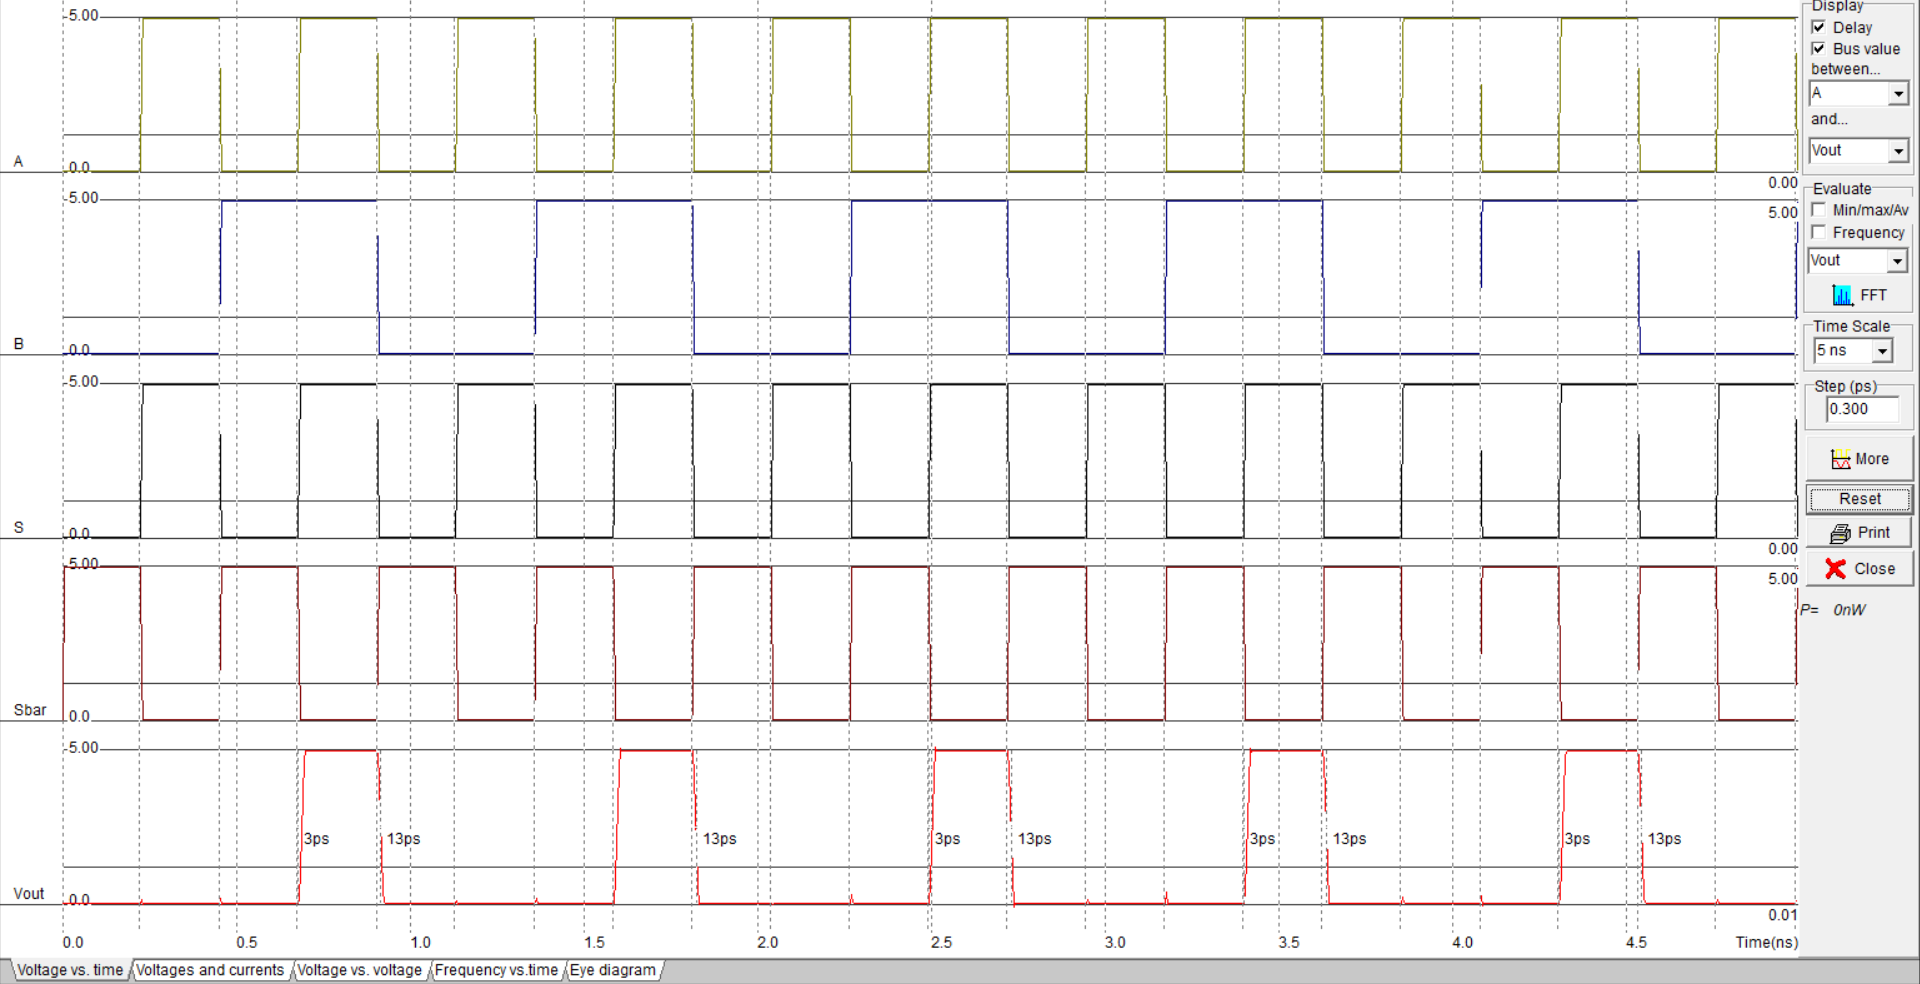
\includegraphics[width=1\linewidth, height=.4\textheight]{Images/2}
		\caption{Output waveshape of 2$\times$1 Multiplexer}
		\label{fig:1}
	\end{figure}
	\begin{figure}[H]
		\centering
	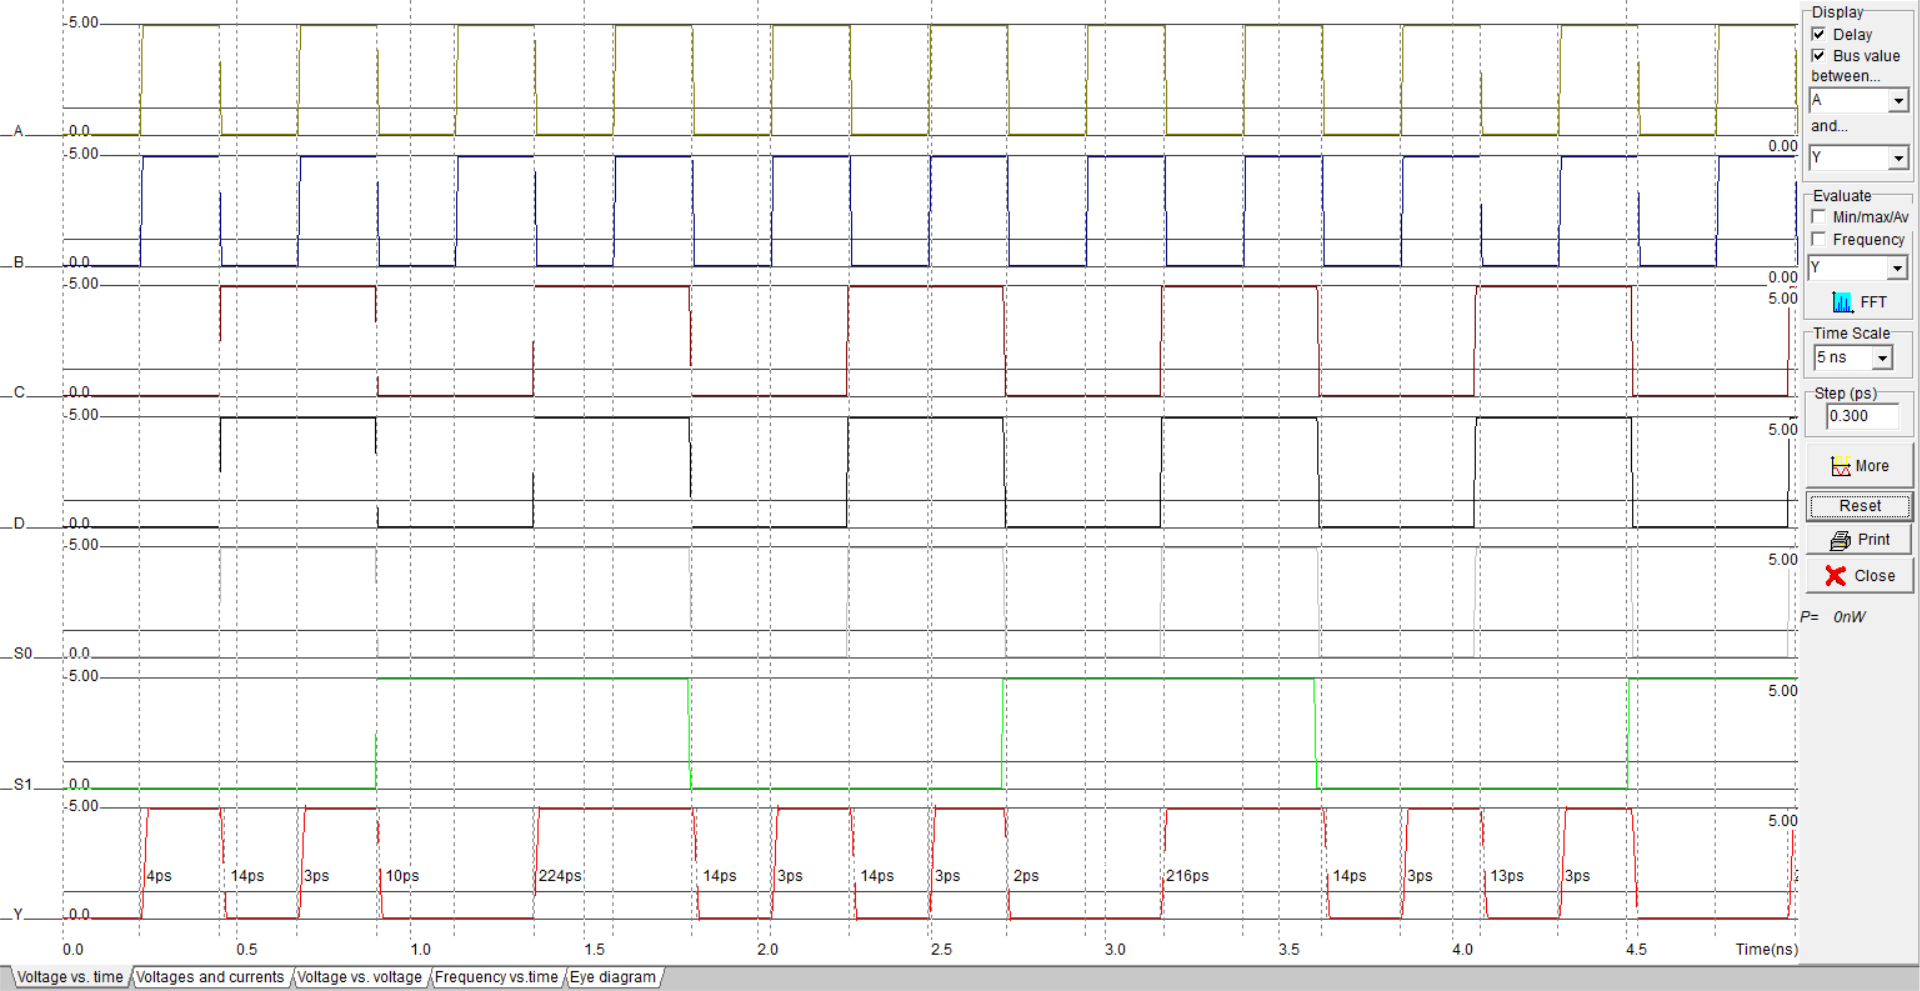
\includegraphics[width=1\linewidth, height=.4\textheight]{Images/4}
		\caption{Output waveshape of 4$\times$1 Multiplexer}
		\label{fig:1}
	\end{figure}
		\begin{figure}[H]
		\centering
		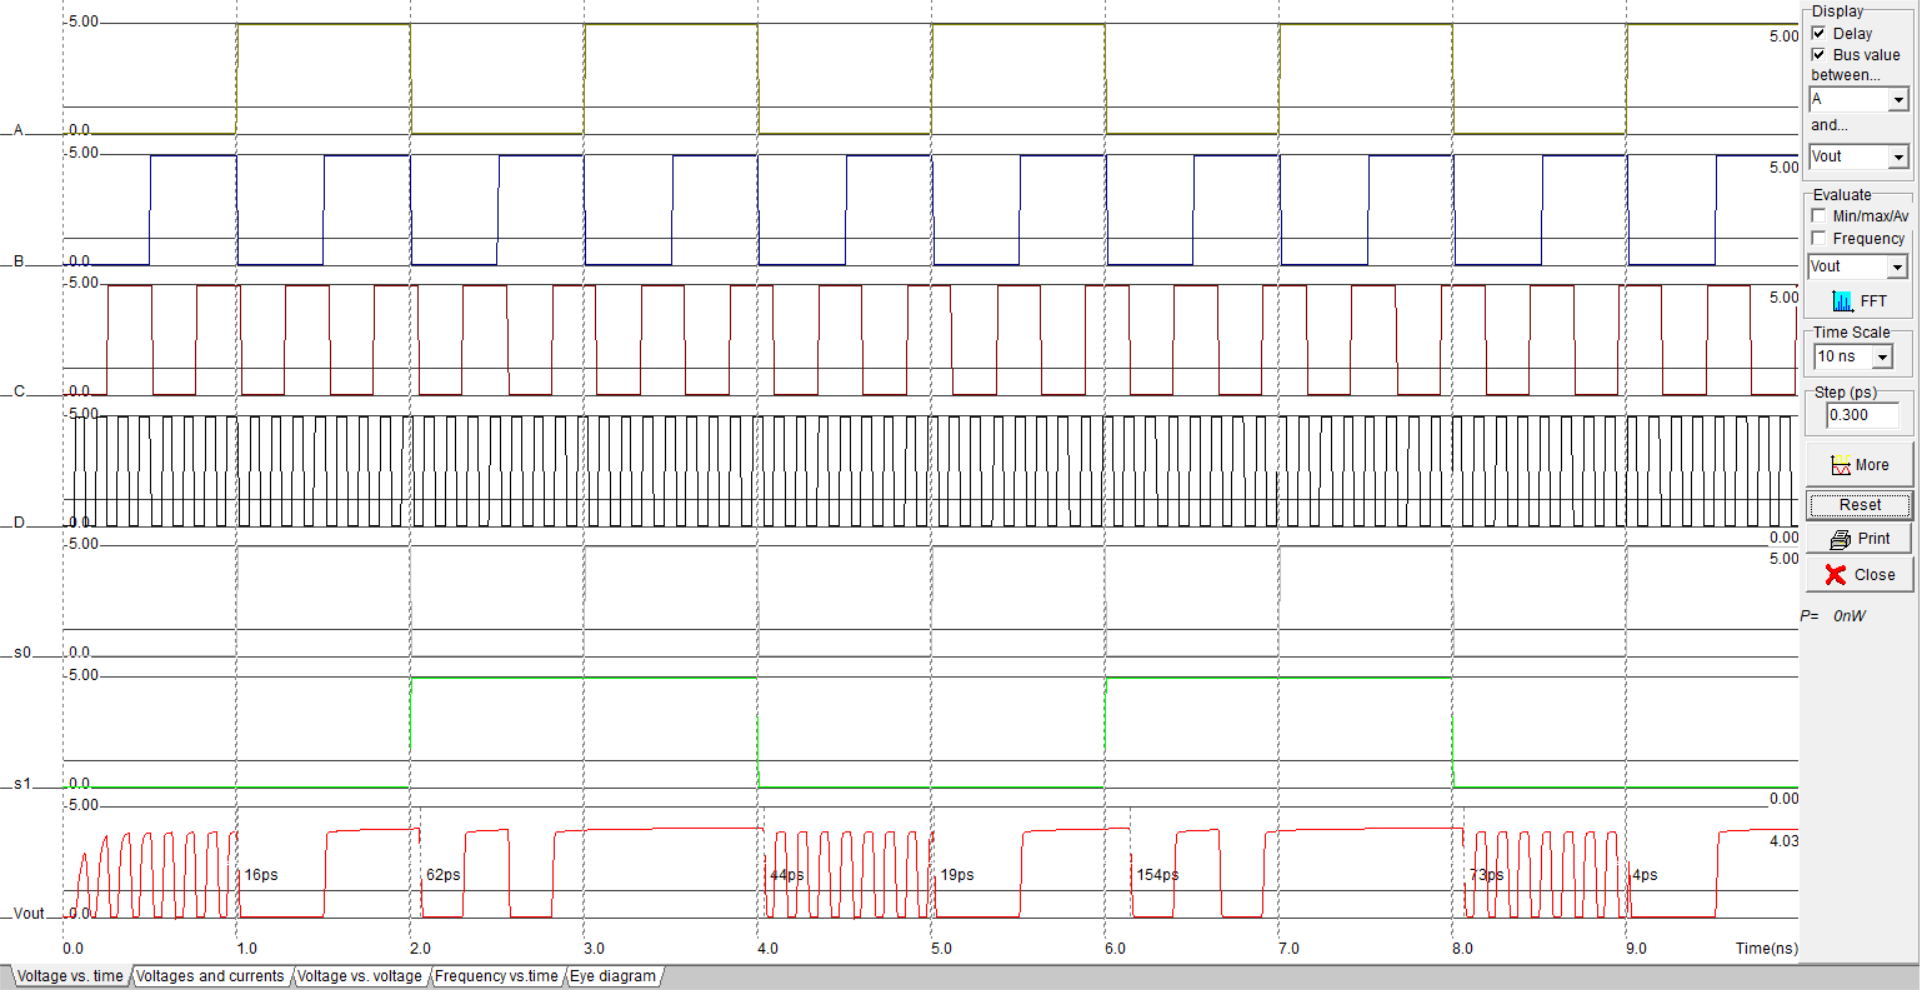
\includegraphics[width=1\linewidth, height=.4\textheight]{Images/5}
		\caption{Output waveshape of 4$\times$1 Multiplexer using nMOS Pass-Transistors}
		\label{fig:1}
	\end{figure}
	
	\section{Discussion }
	In this experiment, 2x1 and 4x1 multiplexers were designed using transmission gates, and the working principle of the transmission gate was analyzed. The circuits were tested under various input conditions to verify their behavior. The input signals were applied to the gates, and the corresponding output responses were observed.
	
	It was noted that for the 2x1 multiplexer, when the control signal \(S_0\) was high, the input signal \(A\) was observed at the output. Conversely, when \(S_0\) was low, the input signal \(B\) appeared at the output, ensuring the correct operation of the 2x1 multiplexer.
	
	On the other hand, for the 4x1 multiplexer, two control signals, \(S_0\) and \(S_1\), were used. For better understanding, the frequencies of input signals \(A\) and \(B\) were set to the same value, and the frequencies of \(C\) and \(D\) were also set to the same value but different from \(A\) and \(B\). Additionally, the frequencies of \(S_0\) and \(S_1\) were taken as double relative to each other to cover all four input conditions. It was clearly observed that the output switched between \(A\), \(B\), \(C\), and \(D\) for different combinations of \(S_0\) and \(S_1\), confirming the correct operation of the 4x1 multiplexer.
	
	The experiment demonstrated the effectiveness of using complementary signals (\(S\) and \(\overline{S}\)) to control the transmission gate. The results obtained were consistent with theoretical expectations, validating the design and functionality of the circuit.
	
	Overall, the practical implementation of the transmission gate and multiplexers was successfully carried out, and their characteristics were thoroughly investigated.
	
	
\end{document}